\documentclass[a4paper, 11pt]{article}
\usepackage{ctex}
\usepackage{amsmath, amssymb}
\usepackage{geometry}
\usepackage{xeCJK}
\usepackage{xeCJKfntef}
\usepackage{ulem}
\usepackage{gensymb}
\usepackage{wrapfig}
\usepackage{graphicx}
\usepackage{fixdif}
\usepackage{fancyhdr}
\usepackage{lastpage}
\usepackage{exam-zh-choices}
\usepackage{exam-zh-question}
\usepackage{exam-zh-textfigure}
\usepackage{tabularray}
\usepackage{multirow}
\usepackage{setspace}

% 页码样式
\pagestyle{fancy} 
\fancyhead{}
\fancyfoot{} 
\fancyfoot[C]{\normalsize 数学试题第\thepage 页(共 \pageref{LastPage} 页)} 
\renewcommand{\headrulewidth}{0mm} % 祛除页眉线

% 定义一些符号
\DeclareMathOperator{\arccot}{arccot}
\newcommand{\dlim}{\displaystyle\lim}
\newcommand{\dint}{\displaystyle\int}
\newcommand{\e}{\mathrm{e}}
\renewcommand{\i}{\mathrm{i}}

\questionsetup{show-answer=true}
\fillinsetup{no-answer-type=none, show-answer=false}

% 页边距
\geometry{
	left=31.7mm, right=31.7mm, top=30.4mm, bottom=30.4mm
}

\begin{document}

\setstretch{1.5}
\begin{center}
	{\fontsize{17pt}{\baselineskip} \selectfont 2024年普通高等学校招生全国统一考试\\[9pt]
		
	\textbf{\fontsize{22pt}{\baselineskip}\selectfont 数\quad 学}}
\end{center}

\noindent\textbf{注意事项:}

1. 答卷前,考生务必将自己的姓名、准考证号填写在答题卡上。

2. 回答选择题时,选出每小题答案后,用铅笔把答题卡上对应题目的答案标号涂黑。如需改动,用橡皮擦干净后,再选涂其他答案标号。回答非选择题时,将答案写在答题卡上。写在本试卷上无效。

3. 考试结束后,将本试卷和答题卡一并交回。\vspace{6pt}

\noindent \textbf{一、选择题:本题共8小题,每小题5分,共40分。在每小题给出的四个选项中,只有一项是符合题目要求的。}\hangindent=2em

\begin{question}
	已知集合$A=\left\{x\mid-5<x^3<5\right\}$, $B=\left\{-3,-1,0,2,3\right\}$,则$A\cap B=$
	\begin{choices}
		\item $\{-1,0\}$
		\item $\{2,3\}$
		\item $\{-3,-1,0\}$
		\item $\{-1,0,2\}$
	\end{choices}
\end{question}

\begin{question}
	若$\dfrac{z}{z-1}=1+\i$,则$z=$
	\begin{choices}
		\item $-1-\i$
		\item $-1+\i$
		\item $1-\i$
		\item $1+\i$
	\end{choices}
\end{question}

\begin{question}
	已知向量$\boldsymbol a=(0,1)$,$\boldsymbol b=(2,x)$,若 $\boldsymbol b\perp (\boldsymbol b-4\boldsymbol a)$,则 $x=$
	\begin{choices}
		\item $-2$
		\item $-1$
		\item $1$
		\item $2$
	\end{choices}
\end{question}

\begin{question}
	已知$\cos(\alpha+\beta)=m$,$\tan\alpha\tan\beta=2$,则 $\cos(\alpha-\beta)=$
	\begin{choices}
		\item $-3m$
		\item $-\dfrac{m}{3}$
		\item $\dfrac{m}{3}$
		\item $3m$
	\end{choices}
\end{question}

\begin{question}
	已知圆柱和圆锥的底面半径相等,侧面积相等,且它们的高均为$\sqrt 3$,则圆锥的体积为
	\begin{choices}
		\item $2\sqrt 3\pi$
		\item $3\sqrt 3\pi$
		\item $6\sqrt 3\pi$
		\item $9\sqrt 3\pi$
	\end{choices}
\end{question}

\begin{question}
	已知函数$f(x)=
	\begin{cases}
		-x^2-2ax-a, &x<0, \\ \e^x+\ln(x+1), &x\geqslant 0
	\end{cases}$在$\mathbb R$上单调递增,则 $a$ 的取值范围是
	\begin{choices}
	\item $(-\infty,0]$
	\item $[-1,0]$
	\item $[-1,1]$
		\item $[0,+\infty)$
	\end{choices}
\end{question}

\begin{question}
	当$x\in[0,2\pi]$时,曲线 $y=\sin x$与 $y=2\sin\left(3x-\dfrac{\pi}{6}\right)$ 的交点个数为
	\begin{choices}
		\item $3$
		\item $4$
		\item $6$
		\item $8$
	\end{choices}
\end{question}

\begin{question}
	已知函数$f(x)$的定义域为 $\mathbb R$, $f(x)>f(x-1)+f(x-2)$,且当 $x<3$时,$f(x)=x$,则下列结论中一定正确的是
	
	\begin{choices}
		\item $f(10)>100$
		\item $f(20)>1\: 000$
		\item $f(10)<1\: 000$
		\item $f(20)<10\: 000$
	\end{choices}
\end{question}

\noindent \textbf{二、选择题:本题共3小题,每小题6分,共18分。在每小题给出的选项中,有多项符合题目要求。全部选对的得6分,部分选对的得部分分,有选错的得0分。}\hangindent=2em

\begin{question}
	为了解推动出口后的亩收入(单位:万元)情况,从该种植区抽取样本,得到推动出口后亩收入的样本均值$\overline{x}=2.1$, 样本方差$s^2=0.01$,已知该种植区以往的亩收入$X$服从正态分布$N\left(1.8, 0.1^2\right)$,假设推动出口后的亩收入$Y$服从正态分布$N\left(\overline{x},s^2\right)$,则(若随机变量$Z$服从正态分布$N\left(\mu,\sigma^2\right)$,则$P(Z<\mu+\sigma)\approx 0.841\: 3$)
		
	\begin{choices}
		\item $P(X>2)>0.2$
		\item $P(X>2)<0.5$
		\item $P(Y>2)>0.5$
		\item $P(Y>2)<0.8$
	\end{choices}
\end{question}

\begin{question}
	设函数$f(x)=\left(x-1\right)^2\left(x-4\right)$,则
	\begin{choices}
		\item $x=3$是 $f(x)$的极小值点
		\item 当$0<x<1$时,$f(x)<f\left(x^2\right)$
		\item 当$1<x<2$时,$-4<f(2x-1)<0$
		\item 当$-1<x<0$时, $f(2-x)>f(x)$
	\end{choices}
	
\end{question}

\textfigure{
	\begin{question}
		造型“
\includegraphics[scale=0.25]{20240608-3.jpg}”可以做成美丽的丝带,将其看作图中曲线$C$的一部分.已知$C$过坐标原点$O$,且$C$上的点满足横坐标大于$-2$,到点$F(2,0)$的距离与到定直线$x=a$ $(a < 0)$的距离之积为$4$,则
		\begin{choices}
			\item $a=-2$
			\item 点$\left(2\sqrt 2,0\right)$在$C$上
			\item $C$在第一象限的点的纵坐标的最大值为$1$
			\item 当点$(x_0,y_0)$在$C$上时, $y_0\leqslant \dfrac{4}{x_0+2}$
		\end{choices}
	\end{question}
}{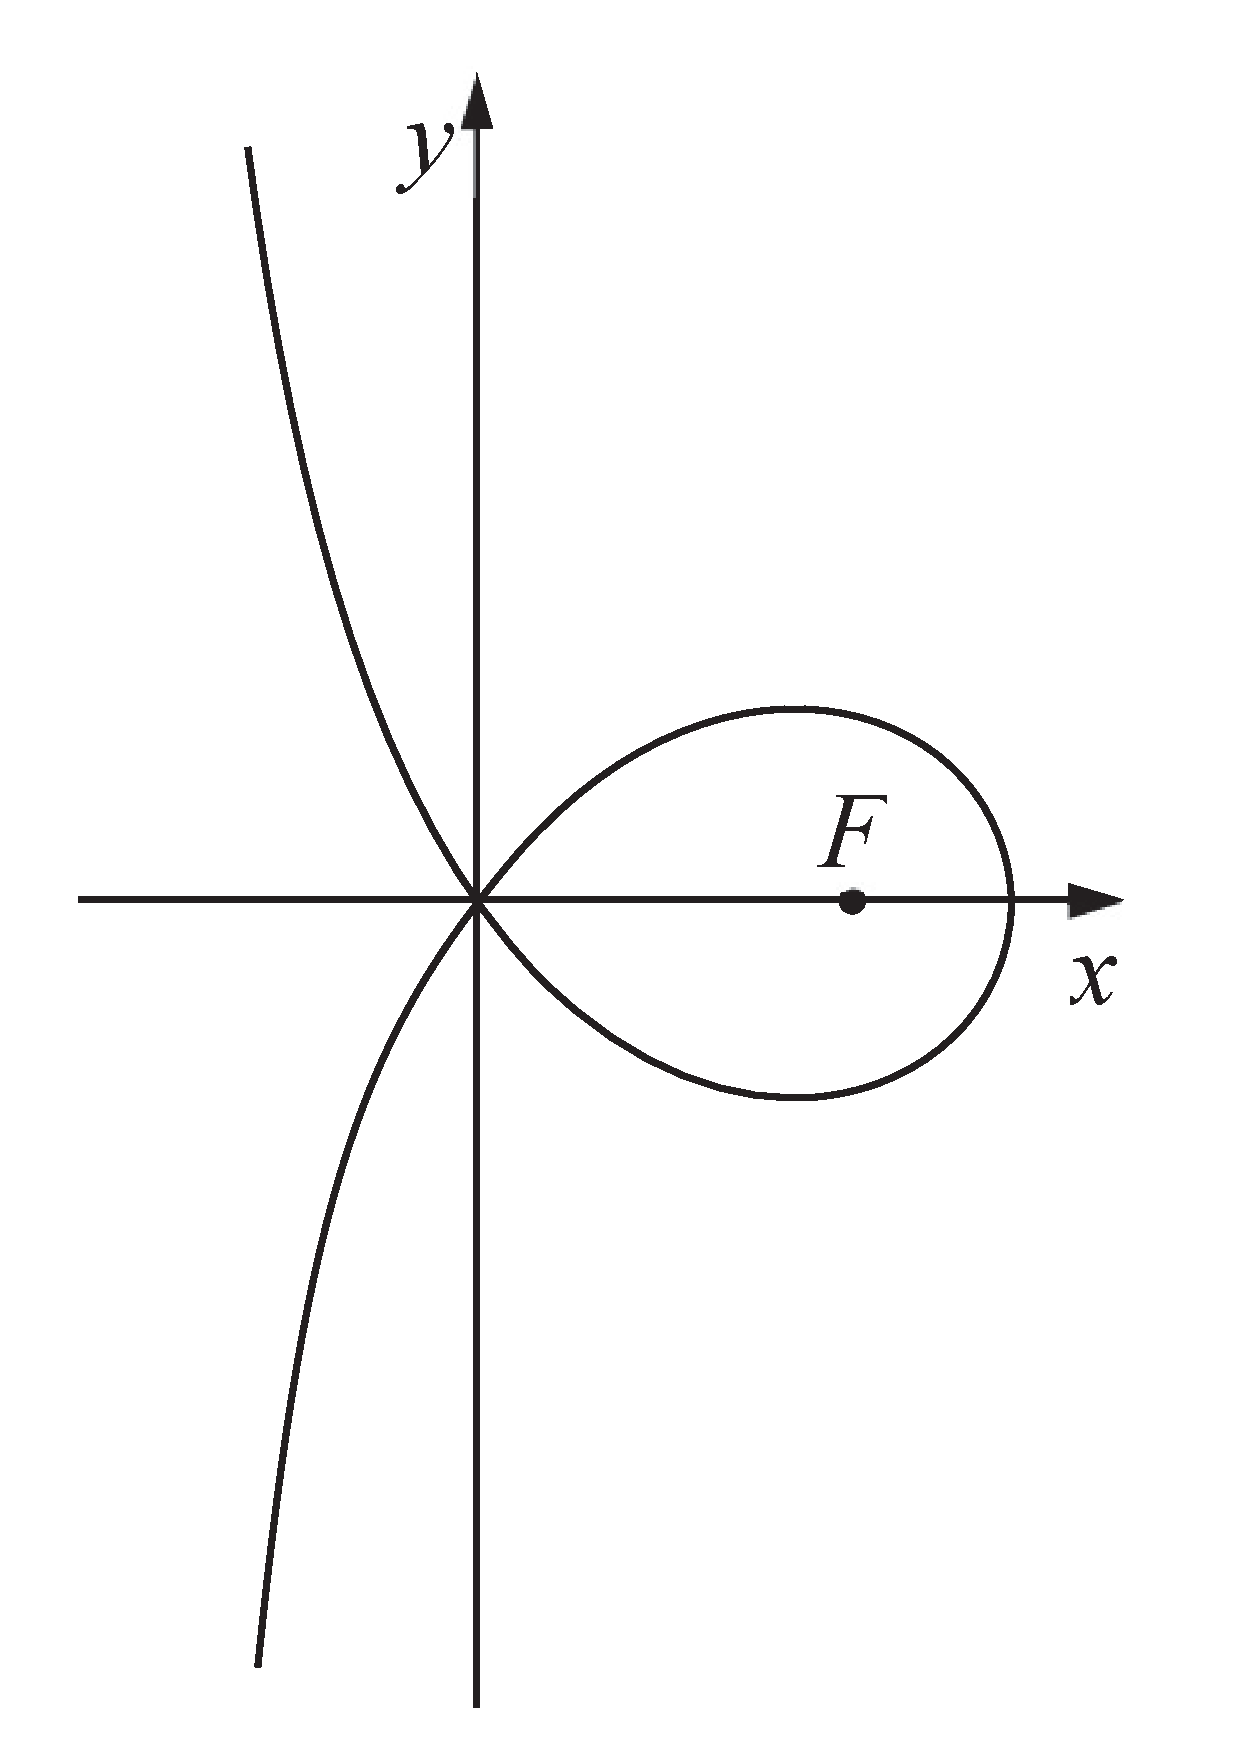
\includegraphics[scale=0.17]{20240608-2.pdf}}

\vspace{10pt}
\noindent \textbf{三、填空题:本题共3小题,每小题5分,共15分。}\hangindent=2em

\begin{question}
	设双曲线$C:\dfrac{x^2}{a^2}-\dfrac{y^2}{b^2}=1$ $(a>0,b>0)$的左、右焦点分别为$F_1$,$F_2$,过$F_2$作平行于$y$轴的直线交 $C$于 $A$、$B$两点,若$\left|F_1A\right|=13$,$\left|AB\right|=10$,则$C$的离心率为\fillin[width=5em][答案].
\end{question}

\begin{question}
	若曲线$y=\e^x+x$在点$(0,1)$处的切线也是曲线$y=\ln(x+1)+a$的切线,则$a=$\fillin[width=5em][答案].
\end{question}

\begin{question}
	甲乙两人各有四张卡片,每张卡片上标有一个数字,甲的卡片上分别标有数字$1$,$3$,$5$,$7$,乙的卡片上分别标有数字$2$,$4$,$6$,$8$.两人进行四轮比赛,在每轮比赛中,两人
各自从自己持有的卡片中随机选一张,并比较所选卡片上的数字大小,数字大的人得$1$分,数字小的人得$0$分,然后各自弃置此轮所选的卡片(弃置的卡片在此后的轮次中不能使用),则四轮比赛后,甲的总得分不小于$2$的概率为\fillin[width=5em][答案]. 
\end{question}


\noindent \textbf{四、解答题:本题共5小题,共77分。解答应写出文字说明、证明过程或演算步骤。}\hangindent=2em

\begin{problem}[points=13]
	设$\triangle ABC$的内角 $A$,$B$,$C$的对边分别为 $a$, $b$, $c$,已知 $\sin C=\sqrt 2\cos B$, $a^2+b^2-c^2=\sqrt 2 ab$.
	
	(1)求$B$;
	
	(2)若$\triangle ABC$的面积为 $3+\sqrt 3$,求 $c$. 
\end{problem}\vspace{80pt}


\begin{problem}[points=15]
	已知$A(0,3)$和 $P\left(3,\dfrac{3}{2}\right)$为椭圆$\dfrac{x^2}{a^2}+\dfrac{y^2}{b^2}=1$ $(a>b>0)$上两点. 
	
	(1)求$C$的离心率;
	
	(2)若过$P$的直线 $l$交 $C$于另一点$B$,且 $\triangle ABP$的面积为 $9$,求 $l$的方程. 
\end{problem}\vspace{80pt}

\textfigure{
	\begin{problem}[points=15]
		如图,四棱锥$P$--$ABCD$中, $PA\perp\text{底面}ABCD$, $PA=AC=2$, $BC=1$, $AB=\sqrt 3$.
		
		(1)若$AD\perp PB$,证明: $AD\parallel\text{平面}PBC$;
		
		(2)若$AD\perp DC$,且二面角 $A$--$CP$--$D$的正弦值为 $\dfrac{\sqrt{42}}{7}$,求$AD$. 
	\end{problem}
}{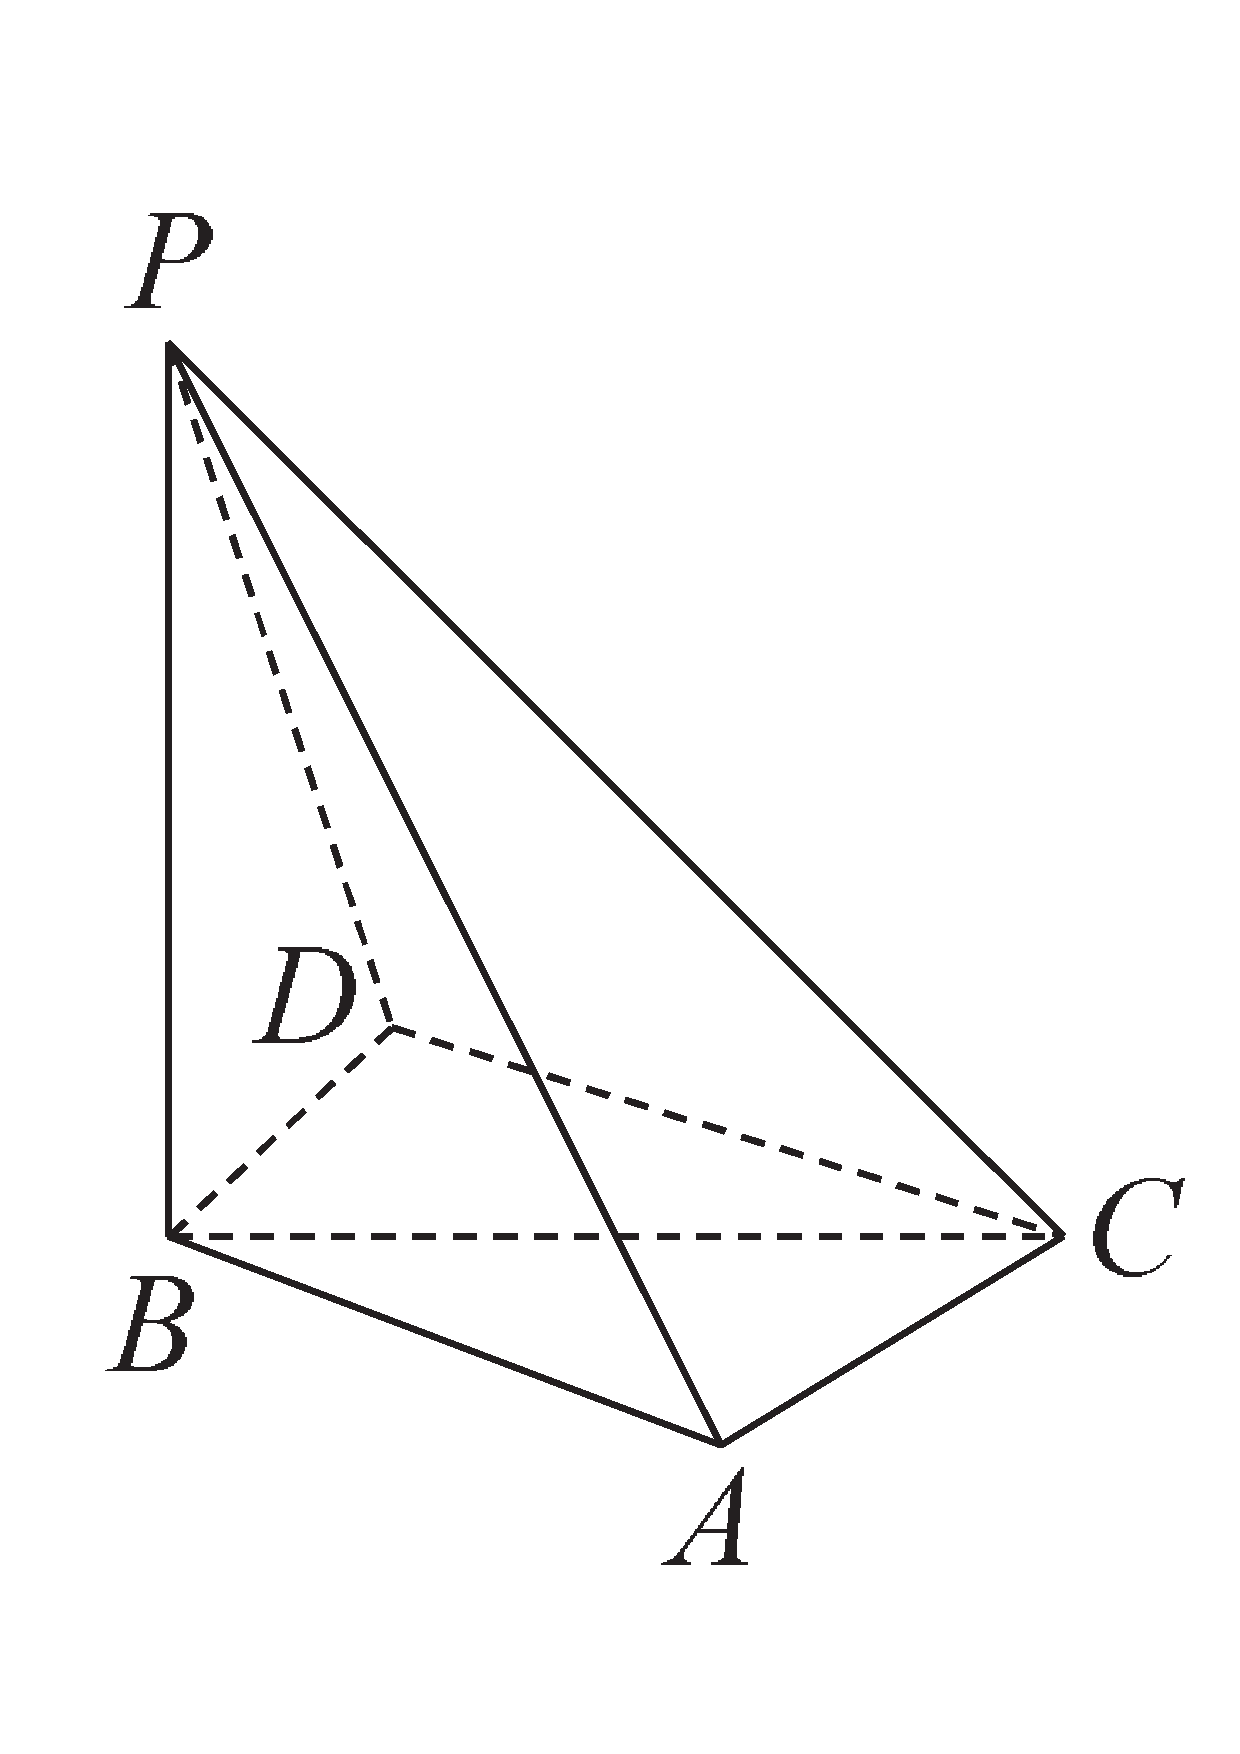
\includegraphics[scale=0.15]{20240608-1.pdf}}

\newpage

\begin{problem}[points=17]
	已知函数$f(x)=\ln \dfrac{x}{2-x}+ax+b\left(x-1\right)^3$. 
	
	(1)若$b=0$,且 $f'(x)\geqslant 0$,求 $a$的最小值;
	
	(2)证明:曲线$y=f(x)$是中心对称图形;

	(3)若 $f(x)>-2$当且仅当 $1<x<2$,求 $b$的取值范围.
\end{problem}\vspace{104pt}

\begin{problem}[points=17]
	设$m$为正整数,数列$a_1$,$a_2$,$\cdots$,$a_{4m+2}$是公差不为$0$的等差数列,若从中删去两项$a_i$和$a_j$ $(i<j)$ 后剩余的$4m$项可被平均分为$m$组,且每组的$4$个数都能构成等差数列,则称数列$a_1$,$a_2$,$\cdots$,$a_{4m+2}$是$(i, j)$--可分数列.
	
	(1)写出所有的$(i,j)$,$1\leqslant i<j\leqslant 6$,使得数列$a_1$,$a_2$,$\cdots$,$a_{6}$是$(i,j)$--可分数列;
	
	(2)当$m\geqslant 3$时,证明:数列$a_1$,$a_2$,$\cdots$,$a_{4m+2}$是$(2,13)$--可分数列;
	
	(3)从$1$,$2$,$\cdots$,$4m+2$中一次任取两个数$i$和$j$ $(i<j)$,记数列$a_1$,$a_2$,$\cdots$,$a_{4m+2}$是$(i,j)$--可分数列的概率为$P_m$,证明:$P_m>\dfrac{1}{8}$.
\end{problem}

\end{document}
